\newcommand\vol{\mathit{vol}}

\chapter{Conductance, Expanders and Cheeger's Inequality}

\sloppy

A common algorithmic problem that arises is the problem of partitioning the vertex set $V$ of a graph $G$ into clusters $X_1, X_2, \dots, X_k$ such that 
\begin{itemize}
    \item for each $i$, the \emph{induced} graph $G[X_i] = (X_i, E \cap (X_i \times X_i))$ is "well-connected", and
    \item only an $\epsilon$-fraction of edges $e$ are not contained in any induced graph $G[X_i]$ (where $\epsilon$ is a very small constant).
\end{itemize}

\begin{figure}[!ht]
    \centering
    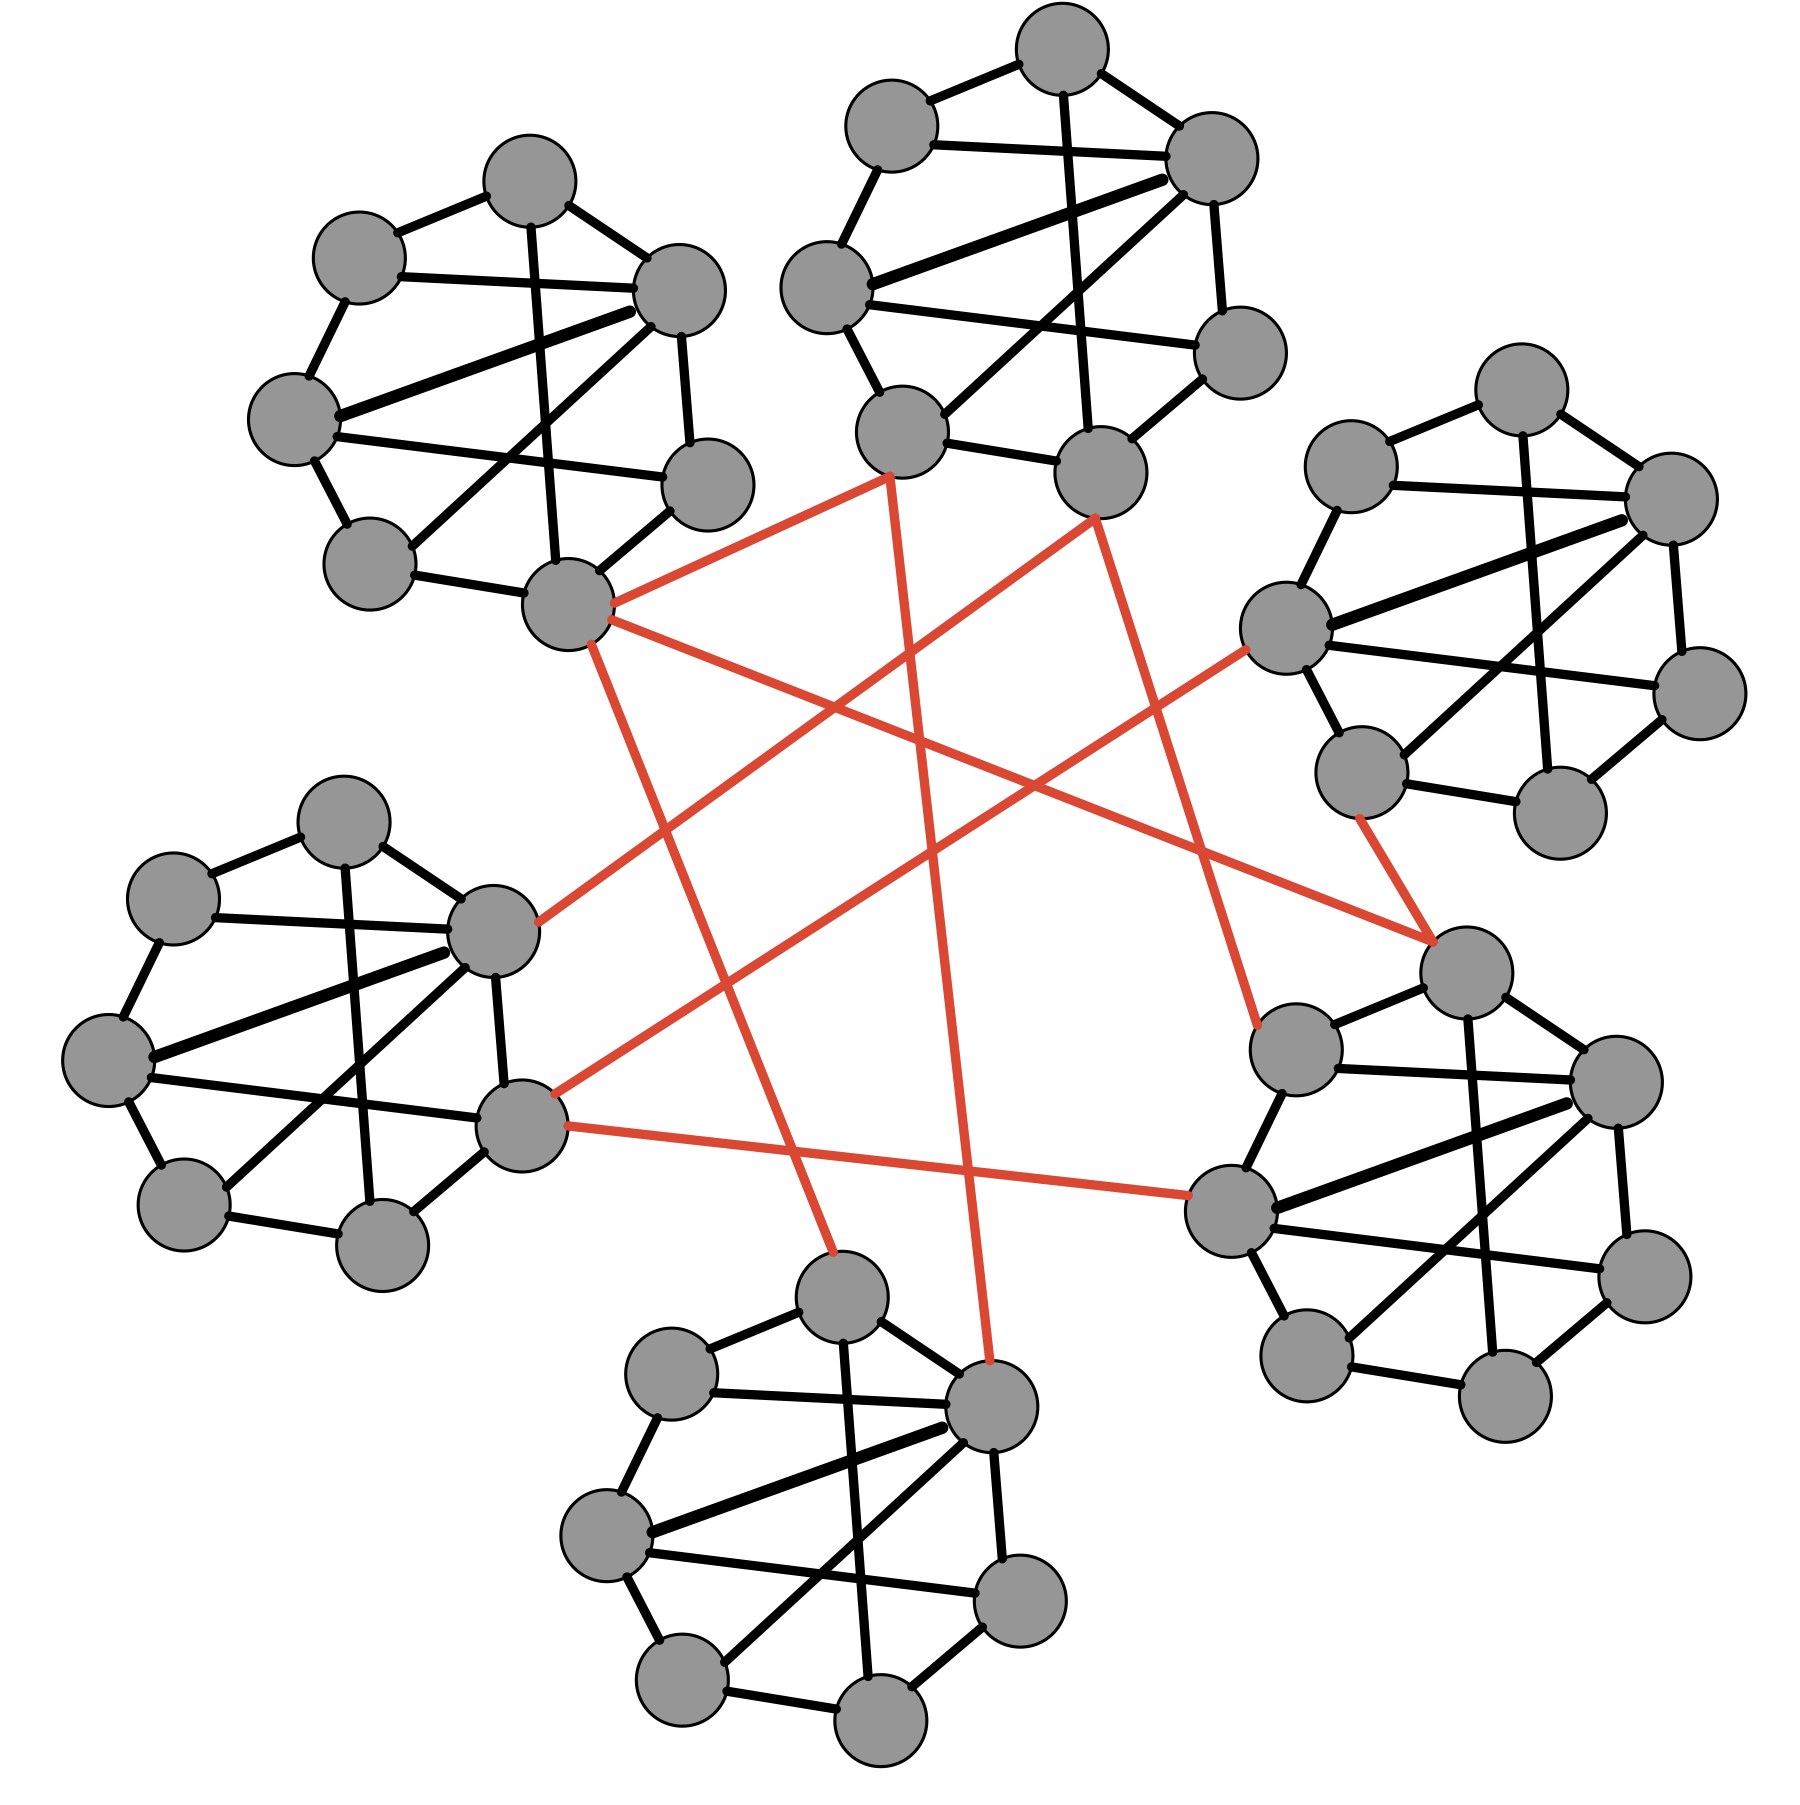
\includegraphics[scale=0.25]{fig/fig1_lecCheeger}
    \caption{After removing the red edges (of which there are few in relation to the total number of edges), each connected component in $G$ is "well-connected".}
\end{figure}

In this lecture, we make precise what "well-connected" means by introducing the notions of \emph{conductance} and \emph{expanders}. 

Building on the last two lectures, we show that the second eigenvalue of the Laplacian $L$ associated with graph $G$ can be used to certify that a graph is "well-connected" (more precisely the second eigenvalue of a normalized version of the Laplacian). This result, called Cheeger's inequality, is one of the key tools in Spectral Graph Theory. Moreover, it can be turned into an algorithm that computes the partition efficiently!

\section{Conductance and Expanders}

\paragraph{Graph Definitions.} In this lecture, we let $G=(V,E)$ be unweighted\footnote{Everything we present here also works for weighted graphs, however, we focus on unweighted graphs for simplicity.} and always be \emph{connected}, and let $\dd(v)$ be the degree of a vertex $v$ in $G$. We define the \emph{volume} $\vol(S)$ for any vertex subset $S \subseteq V$, to be the sum of degrees, i.e. $\vol(S) = \sum_{v \in S} \dd(v)$.

For any  $A, B \subseteq V$, we define $E(A, B)$ to be the set of edges in $E \cap (A \times B)$, i.e. with one endpoint in $A$ and one endpoint in $B$. We let $G[A]$ be the \emph{induced} graph $G$ by $A \subseteq V$, which is the graph $G$ restricted to the vertices $A$, i.e. an edge $e$ in $G$ is in $G[A]$ iff both endpoints are in $A$.

\paragraph{Conductance.} Given set $\emptyset \subset S \subset V$, then we define the conductance $\phi(S)$ of $S$ by
\[
\phi(S) = \frac{|E(S, V \setminus S)|}{ \min\{\vol(S), \vol(V \setminus S) \} }.
\]
It can be seen that $\phi(\cdot)$ is symmetric in the sense that $\phi(S) = \phi(V \setminus S)$. We define the conductance of the graph $G$ denoted $\phi(G)$ by
\[
    \phi(G) = \min_{\emptyset \subset S \subset V} \phi(S). 
\]
We note that finding the conductance of a graph $G$ is NP-hard. However, good approximations can be found as we will see today (and in a later lecture).

\paragraph{Expander and Expander Decomposition.} For any $\phi \in (0, 1]$, we say that a graph $G$ is a \emph{$\phi$-expander} if $\phi(G) \geq \phi$. We say that the partition $X_1, X_2, \dots, X_k$ of the vertex set $V$ is a \emph{$\phi$-expander decomposition} of quality $q$ if
\begin{itemize}
    \item each induced graph $G[X_i]$ is a $\phi$-expander, and
    \item the number of edges not contained in any $G[X_i]$ is at most $q \cdot \phi \cdot m$.
\end{itemize}
Today, we obtain a $\phi$-expander decomposition of quality $q = O(\phi^{-1/2} \cdot \log n)$. In a few lectures, we revisit the problem and obtain quality $q = O(\log^c n)$ for some small constant $c$. In practice, we mostly care about values $\phi \approx 1$.

\paragraph{An Algorithm to Compute Conductance and Expander Decomposition.} 
In this lecture, the main focus is \emph{not} to obtain an algorithm to compute conductance but rather only to show that the conductance of a graph can be approximated using the eigenvalues of the "normalized" Laplacian. 

However, this proof gives then rise to an algorithm $\textsc{CertifyOrCut}(G, \phi)$ that given a graph $G$ and a parameter $\phi$ either: 
\begin{itemize}
    \item \emph{Certifies} that $G$ is a $\phi$-expander, or
    \item Presents a \emph{cut} $S$ such that $\phi(S) \leq \sqrt{2\phi}$.
\end{itemize}
In the graded homework, we ask you to make the procedure $\textsc{CertifyOrCut}(G, \phi)$ explicit, and then to show how to use it to compute a $\phi$-expander decomposition. 

\section{A Lower Bound for Conductance via Eigenvalues}

\paragraph{An Alternative Characterization of Conductance.} Let us now take a closer look at the definition of conductance and observe that if a set $S$ has $\vol(S) \leq \vol(V)/2$ then
\[
\phi(S) = \frac{|E(S, V \setminus S)|}{ \min\{\vol(S), \vol(V \setminus S)\} } = \frac{|E(S, V \setminus S)|}{ \vol(S) } = \frac{\vecone_S^\trp \LL \vecone_S}{\vecone_S^\trp \DD \vecone_S}.
\]
To see this, observe that we can rewrite the numerator above using the Laplacian of $G$ as
\[
|E(S, V \setminus S)| = \sum_{(u,v)\in E} (\vecone_S(u) - \vecone_S(v))^2 =  \vecone_S^\trp \LL \vecone_S
\]
where $\vecone_S$ is the characteristic vector of $S$. Further, we can rewrite the denominator as 
\[
\vol(S) = \vecone_S^\trp \dd = \vecone_S^\trp \DD \vecone_S
\]
where $\DD = \diag(\dd)$ is the degree-matrix. We can now alternatively define the graph conductance of $G$ by
\begin{equation}\label{eq:conductanceAltDef}
\phi(G) = \min_{\stackrel{\emptyset \subset S \subset V,} {\vol(S) \leq \vol(V)/2}} \frac{\vecone_S^\trp \LL \vecone_S}{\vecone_S^\trp \DD \vecone_S} 
\end{equation}
where we use that $\phi(S) = \phi(V \setminus S)$ such that the objective value is unchanged as long as for each set $\emptyset \subset S \subset V$ either $S$ or $V \setminus S$ is in the set that we minimize over.

\paragraph{The Normalized Laplacian.} Let us next define the \emph{normalized} Laplacian \[
\NN = \DD^{-1/2} \LL \DD^{-1/2} = \II -  \DD^{-1/2} \AA \DD^{-1/2}.
\]
To learn a bit about this new matrix, let us first look at the first eigenvalue where we use the test vector $y = \DD^{1/2}\vecone$, to get by Courant-Fischer (see \Cref{thm:courant-fischer-eigvec}) that
\begin{align}\label{eq:plugInNormalizedVector}
    \lambda_1(\NN) =
    \min_{
      \substack{ \xx \neq \veczero}
    }
    \frac{\xx^\trp \NN\xx}{\xx^\trp\xx}  \leq \frac{\yy^\trp\DD^{-1/2} \LL \DD^{-1/2} \yy}{\yy^\trp\yy} = \frac{\vecone^\trp \LL \vecone}{\yy^\trp\yy} = 0
\end{align}
because $\DD^{-1/2} \DD^{1/2} = I$ and $\LL \vecone = 0$ (for the former we use the assumption that $G$ is connected). Since $\NN$ is PSD (as you will show in the exercises), we also know $\lambda_1(\NN) \geq 0$, so $\lambda_1(\NN) = 0$.

Let us use Courant-Fischer again to reason a bit about the second eigenvalue of $\NN$:
\begin{align}\label{eq:courantFisherSecondEig}
    \lambda_2(\NN) =
    \min_{
      \substack{ \xx \perp \DD^{1/2}\vecone \\ \xx \neq \veczero}
    }
    \frac{\xx^\trp \NN\xx}{\xx^\trp\xx} = 
    \min_{
      \substack{ \zz \perp \dd \\ \zz \neq \veczero}
    }
    \frac{\zz^\trp \DD^{1/2}  \NN \DD^{1/2} \zz}{\zz^\trp \DD^{1/2}\DD^{1/2}\zz} = \min_{
      \substack{ \zz \perp \dd \\ \zz \neq \veczero}
    } \frac{\zz^\trp \LL \zz}{\zz^\trp \DD \zz}.
\end{align}

\paragraph{Relating Conductance to the Normalized Laplacian.} At this point, it might become clearer why $\NN$ is a natural matrix to consider when arguing about conductance: if we could argue that for every $\emptyset \subset S \subset V, \vol(S) \leq \vol(V)/2$, we have $\vecone_S \perp \dd$, then it would be easy to see that taking the second eigenvalue of $\NN$ in equation \ref{eq:courantFisherSecondEig} is a relaxation of the minimization problem \ref{eq:conductanceAltDef} defining $\phi(G)$.

While this is clearly not true, we can still argue along these lines.

\begin{theorem}[Cheeger's Inequality, Lower Bound]\label{thm:cheegerInequLowerBound}
We have $\frac{\lambda_2(\NN)}{2} \leq \phi(G)$.
\end{theorem}
\begin{proof}
Instead of using $\vecone_S$ directly, we shift $\vecone_S$ by $\vecone$ such that it is orthogonal to $\dd$: we define $\zz_S = \vecone_S - \alpha \vecone$ where $\alpha$ is the scalar that solves
\begin{align*}
       0 &= \dd^\trp \zz_S \\
       \iff 0 &= \dd^\trp(\vecone_S - \alpha \vecone)\\
       \iff 0 &= \dd^\trp \vecone_S - \alpha  \dd^\trp\vecone \\
       \iff \alpha &= \frac{\dd^\trp \vecone_S}{\dd^\trp\vecone} = \frac{\vol(S)}{\vol(V)}.
\end{align*}

To conclude the proof, it remains to argue that $\frac{\vecone_S^\trp \LL \vecone_S}{\vecone_S^\trp\DD\vecone_S} \geq \frac{1}{2} \cdot \frac{\zz_S^\trp \LL \zz_S}{\zz_S^\trp\DD\zz_S}$:
\begin{itemize}
    \item Numerator: since $\vecone^\trp \LL \vecone = 0$, we have that $\vecone_S^\trp \LL \vecone_S = \zz_S^\trp \LL \zz_S$.
    \item Denominator: observe by straight-forward calculations that \begin{align*}
        \zz_S^\trp\DD\zz_S &= \vol(S) \cdot (1-\alpha)^2 + \vol(V \setminus S) \cdot (-\alpha)^2\\
        &= \vol(S) - 2\vol(S) \cdot \alpha + \vol(V) \cdot \alpha^2\\
        & = \vol(S) -   \frac{\vol(S)^2}{\vol(V)} \\
        & = \vol(S) - \vol(S) \cdot  \frac{\vol(S)}{\vol(V)}\\
        & \geq \frac{1}{2}\vol(S) = \frac{1}{2}\vecone_S^\trp\DD\vecone_S
    \end{align*}
    where we use the assumption that $\vol(S) \leq \vol(V)/2$.
\end{itemize}
\end{proof}

\section{An Upper Bound for Conductance via Eigenvalues}

Slightly more surprisingly, we can also show that the second eigenvalue $\lambda_2(\NN)$ can be used to upper bound the conductance.

\begin{theorem}[Cheeger's Inequality, Upper Bound]\label{thm:cheegerInequUpperBound}
We have $\phi(G) \leq \sqrt{2 \cdot \lambda_2(\NN)}$.
\end{theorem}
\begin{proof}
To prove the theorem, we want to show that for \emph{any} $\zz \perp \dd$, we can find a set $\emptyset \subset S \subset V$, such that 
\begin{equation}\label{eq:findTightCutCheeger}
\frac{\vecone_S^\trp \LL \vecone_S}{\vecone_S^\trp \DD \vecone_S}  \leq \sqrt{2 \cdot \frac{\zz^\trp \LL \zz}{\zz^\trp \DD \zz}}.    
\end{equation}

As a first step, we would like to change $\zz$ slightly to make it more convenient to work with:
\begin{itemize}
    \item we \emph{renumber} the vertices in $V$ such that we have
    \[
    \zz(1) \leq \zz(2) \leq \dots \leq \zz(n).
    \]
    \item we \emph{center} $\zz$, that is we let $\zz_c = \zz - \alpha \vecone$ where $\alpha$ is chosen such that \begin{align*}
        \sum_{\zz_c(i) < 0} \dd(i) < \vol(V)/2 \text{ and }
        \sum_{\zz_c(i) \leq 0} \dd(i) \geq \vol(V)/2
    \end{align*}
    i.e. $\sum_{\zz_c(i) > 0} \dd(i) \leq \vol(V)/2$.
    \item we \emph{scale}, let $\zz_{sc} = \beta \zz_c$ for some scalar $\beta$ such that $\zz_{sc}(1)^2 + \zz_{sc}(n)^2 = 1$. 
\end{itemize}
In the exercises, you will show that changing $\zz$ to $\zz_{sc}$ can only make the ratio we are interested in smaller, i.e. that
$\frac{\zz^\trp \LL \zz}{\zz^\trp \DD \zz} \geq \frac{\zz_{sc}^\trp \LL \zz_{sc}}{\zz_{sc}^\trp \DD \zz_{sc}}$. Thus, if we can show that equation \ref{eq:findTightCutCheeger} holds for $\zz_{sc}$ in place of $\zz$, then it also follows for $\zz$ itself.

We now arrive at the main idea of the proof: we define the set $S_{\tau} = \{ i \in V \;|\; \zz_{sc}(i) < \tau\}$ for some random variable $\tau$ with distribution with probability density function
\begin{align}\label{eq:cheegerDefineDensityFun}
    p(t) = \begin{cases}
        2 \cdot |t| &t \in [\zz_{sc}(1), \zz_{sc}(n)],
        \\
        0 &\text{otherwise}.
        \end{cases}
\end{align}
So, we have probability $\mathbb{P}[a < \tau < b] = \int_{t=a}^b p(t)\; dt$.

Since the volume incident to $S_{\tau}$ might be quite large, let us define $S$ for convenience by
\[
S = \begin{cases}
        S_{\tau} & \vol(S_{\tau}) < \vol(V)/2,
        \\
        V \setminus S_{\tau} &\text{otherwise}.
        \end{cases}
\]

\begin{claim}\label{clm:cheegersInequInExpectation}
We have  $\frac{\mathbb{E}_{\tau}\left[\vecone_S^\trp \LL \vecone_S\right]}{\mathbb{E}_{\tau}\left[{\vecone_S^\trp \DD \vecone_S}  \right]} \leq \sqrt{2 \cdot \frac{\zz_{sc}^\trp \LL \zz_{sc}}{\zz_{sc}^\trp \DD \zz_{sc}}}$.
\end{claim}
\begin{proof}
Recall $\vecone_S^\trp \LL \vecone_S = E(S_{\tau}, V \setminus S_{\tau})$, and by choice of $\tau$, we have for any edge $e = \{i,j\} \in E$ where $\zz_{sc}(i) \leq \zz_{sc}(j)$,
\begin{align*}
    \mathbb{P}_{\tau}[e \in E(S_{\tau}, V \setminus S_{\tau})] &= \mathbb{P}_{\tau}[\zz_{sc}(i) < \tau \leq \zz_{sc}(j)] \\ &= \int_{t=i}^j 2|t|\; dt = \sgn{j} \cdot \zz_{sc}(j)^2 - \sgn{i} \cdot \zz_{sc}(i)^2.
\end{align*}
Distinguishing by cases, we get
\[
\sgn{j} \cdot \zz_{sc}(j)^2 - \sgn{i} \cdot \zz_{sc}(i)^2 = \begin{cases}
    |\zz_{sc}(i)^2 - \zz_{sc}(j)^2| & \sgn{i} = \sgn{j},
    \\
    \zz_{sc}(i)^2 + \zz_{sc}(j)^2 &\text{otherwise}.
    \end{cases} 
\]
We can further upper bound either case by $ |\zz_{sc}(i) - \zz_{sc}(j)| \cdot (|\zz_{sc}(i)| + |\zz_{sc}(j)|)$ (we leave this as an exercise).

Using our new upper bound, we can sum over all edges $e \in E$ to conclude that
\begin{align*}
   \mathbb{E}_{\tau}[|E(S_{\tau}, V \setminus S_{\tau})|] &\leq \sum_{i \sim j} |\zz_{sc}(i) - \zz_{sc}(j)| \cdot (|\zz_{sc}(i)| + |\zz_{sc}(j)|) \\
   &\leq \sqrt{\sum_{i \sim j} (\zz_{sc}(i) - \zz_{sc}(j))^2 \cdot \sum_{i \sim j} (|\zz_{sc}(i)| + |\zz_{sc}(j)|)^2 }
\end{align*}
where the last line follows from $\langle \xx, \yy \rangle^2 \leq \langle \xx, \xx \rangle \cdot \langle \yy, \yy \rangle$ (i.e. Cauchy-Schwarz).\\

The first sum should look familiar by now: it is simply the Quadratic Laplacian Form $\sum_{i \sim j} (\zz_{sc}(i) - \zz_{sc}(j))^2 = \zz_{sc}^\trp \LL \zz_{sc}$. \\

It is not hard to reason about the second term either
\[
\sum_{i \sim j} (|\zz_{sc}(i)| + |\zz_{sc}(j)|)^2 \leq 2\sum_{i \sim j} \zz_{sc}(i)^2 + \zz_{sc}(j)^2 = 2\sum_{i \in V} \dd(i) \zz_{sc}(i)^2 = 2 \zz_{sc}^{\trp} \DD \zz_{sc}.
\]

Putting everything together, we obtain
\begin{align}\label{eq:cheegerInequAlmostDone}
   \mathbb{E}_{\tau}[|E(S_{\tau}, V \setminus S_{\tau})|] \leq \sqrt{\zz_{sc}^\trp \LL \zz_{sc} \cdot 2 \zz_{sc}^{\trp} \DD \zz_{sc}} = \sqrt{2 \cdot \frac{\zz_{sc}^\trp \LL \zz_{sc}}{\zz_{sc}^{\trp} \DD \zz_{sc}} }\; \cdot \; \zz_{sc}^{\trp} \DD \zz_{sc}
\end{align}

While this almost looks like what we want, we still have to argue that $\zz_{sc}^\trp \DD \zz_{sc} = \mathbb{E}_{\tau}[\vecone_S^\trp \DD \vecone_S]$ to finish the proof.

To this end, when unrolling the expectation, we use a simple trick that splits by cases:
\begin{align*}
    \mathbb{E}_{\tau}[\vecone_S^\trp \DD \vecone_{S}] &=\sum_{i \in V} \dd(i) \cdot \mathbb{P}[i \in S] \\
    &=\sum_{i \in V, \zz_{sc}(i) < 0} \dd(i) \cdot \mathbb{P}[i \in S \land S=S_{\tau}] + \sum_{i \in V, \zz_{sc}(i) \geq 0} \dd(i) \cdot \mathbb{P}[i \in S \land S \neq S_{\tau}]\\
     &=\sum_{i \in V, \zz_{sc}(i) < 0} \dd(i) \cdot \mathbb{P}[\zz_{sc}(i) < \tau \land \tau < 0] + \sum_{i \in V, \zz_{sc}(i) \geq 0} \dd(i) \cdot \mathbb{P}[\zz_{sc}(i) \geq \tau \land \tau \geq 0]
\end{align*}
where we use the centering of $\zz_{sc}$ the definition of $S$ and that the event $\{i \in S \land S=S_{\tau}\}$ can be rewritten as the event $\{i < \tau \land \tau < 0\}$ (the other case is analogous). 

Let $i$ be a vertex with $\zz_{sc}(i) < 0$, then the probability $\mathbb{P}[i \in S \land S=S_{\tau}]$ is exactly $\zz_{sc}(i)^2$ by choice of the density function of $\tau$ (again the case for $i$ with $\zz_{sc}(i)$ non-negative is analgous). Thus, summing over all vertices, we obtain 
\begin{align*}
    \mathbb{E}_{\tau}[\vecone_S^\trp \DD \vecone_{S}] 
     &=\sum_{i \in V, \zz_{sc}(i) < 0} \dd(i) \cdot \mathbb{P}[\zz_{sc}(i) < \tau \land \tau < 0] + \sum_{i \in V, \zz_{sc}(i) \geq 0} \mathbb{P}[\zz_{sc}(i) \geq \tau \land \tau \geq 0]\\
     & = \sum_{i \in V } \dd(i) \cdot \zz_{sc}(i)^2 = \zz_{sc}^\trp \DD \zz_{sc}.
\end{align*}
Therefore, we can plug in our result directly into Equation 
\ref{eq:cheegerInequAlmostDone} and the proof is completed by dividing both sides by $\mathbb{E}_{\tau}[\vecone_S^\trp \DD \vecone_{S}]$. 
\end{proof}

While \Cref{clm:cheegersInequInExpectation} only ensures our claim in expectation, this is already sufficient to conclude that there exists some set $S$ that satisfies the same guarantees deterministically, as you will prove in Problem Set 4. This is often called the \emph{probabilistic method of expectation} and can be seen from the definition of expectation. We have thus proven the upper bound of Cheeger's inequality.
\end{proof}

\section{Conclusion}

Today, we have introduced the concepts of conductance and formalized expanders and expander decompositions. These are crucial concepts that you will encounter often in literature and also again in this course. They are a key tool in many recent breakthroughs in Theoretical Computer Science.

In the second part of the lecture (the main part), we discussed Cheeger's inequality which allows to relate the second eigenvalue of the normalized Laplacian to a graphs conductance. We summarize the full statement here.

\begin{theorem}[Cheeger's Inequality]\label{thm:cheegerInequFull}
We have $\frac{\lambda_2(\NN)}{2} \leq \phi(G) \leq \sqrt{2 \cdot \lambda_2(\NN)}$.
\end{theorem}

We point out that this Theorem is tight as you will show in the exercises. The proof for Cheeger's inequality is probably the most advanced proof, we have seen so far in the course. The many tricks that make the proof work might sometimes seem a bit magical but it is important to remember that they are a result of many people polishing this proof over and over. The proof techniques used are extremely useful and can be re-used in various contexts. We therefore strongly encourage you to really understand the proof yourself!
